\section{ОБЗОР ЛИТЕРАТУРЫ}
\label{sec:domain}

\subsection{Брокеры сообщений}

Для передачи данных между компонентами в сложной системе используются так называемые брокеры сообщений (англ. message broker).
Это программа, целью которой является приём, хранение и передача сообщений.
Традиционно брокер состоит из следующих компонентов:
\begin{itemize}
    \item Сообщения - совокупность двоичных или текстовых данных, имеющих что-то общее в контексте программы.
     К этим данным перед отправкой может добавляться дополнительная информация, в зависимости от протокола.
    \item Очереди сообщений - объекты, хранящие сообщения в программе;
\end{itemize}

Существует множество брокеров сообщений. Наиболее известные из них:
\begin{itemize}
    \item ActiveMQ;
    \item IBM MQ;
    \item RabbitMQ;
    \item Redis;
    \item Kafka.
\end{itemize}


Сегодня все больше и больше встраиваемых систем окружают нас. «Умная» бытовая
техника, повсеместные системы видеонаблюдения -- и этот список еще можно
продолжать и продолжать. При этом, большинству этих систем требуется максимально
быстро реагировать на воздействия (например, система видеонаблюдения должна начать
запись при обнаружении движения).
Из-за этого, разработчкики вынуждены использовать операционные системы
реального времени. В отличие от других типов операционных систем (пакетных и
интерактивных), основная часть задач выполняется достаточно быстро, чтобы
не задерживать работу остальных компонентов ~\cite{tanenbaum_modern_os_2015_ru}.
% Таненбаум Modern OS 2015 RUS, страница 183
Остальным задачам задают низкий приоритет, что позволяет им работать в фоновом
режиме и практически не влиять на работу высокоприоритетных задач.

Операционные системы реального времени имеют еще ряд особенностей
~\cite{tanenbaum_modern_os_2015_ru},~\cite{rtos_valvano}:
\begin{itemize}
    \item временные ограничения на обработку данных;
    \item предсказуемость поведения во времени;
    \item простота внутренней реализации.
\end{itemize}

Временные органичения на обработку данных подразумевают, что скорость обработки
данных составляет не меньше скорости их поступления. Это обусловлено тем, что
система должна полностью обработать данные до поступления новой порции, поскольку
если такого не будет происходить, необработанные данные будут накапливаться,
что приведет к затору.

Иногда системы реального времени допускают частичные заторы путем отбрасывания
необработанных данных. В зависимости от типа обрабатываемой информации
может быть разрешена разная степень игнорирования входных данных
~\cite{tanenbaum_modern_os_2015_ru}.

Простота внутренней реализации связана с тем, что обычно данная
операционная система не программируется извне (конечным пользователем).
Поэтому она не требует поддержки расширяемости во время исполнения,
различных уровней привелегий, имеет более примитивную внутреннюю структуру
и, обычно, ей практически не требуется время для запуска ~\cite{rtos_valvano}.
% Valvano page 19

Отсюда также следуют и различия в архитектуре. Архитектура операционной системы
реального времени упрощена, из нее убраны излишние слои.
Она визуально отмечена на рисунке~\ref{pic:lit_review:rtos_arch} желтым цветом.
Зеленым цветом отмечено управляющий микропроцессор или микроконтроллер, который
исполняет код, а также периферийные устройства, которые предназначены
для ввода и вывода информации. Красным отмечено приложение. Оно
управляет аппаратным обеспечением (зеленой компонентой) с помощью операционной
системы реального времени (желтой компоненты) ~\cite{rtos_arch_site}.

\aconstskip\begin{figure}
    \centering
    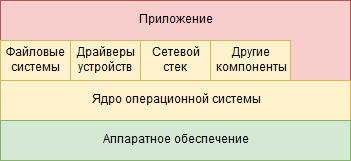
\includegraphics[width=0.7\textwidth]{RTOS_architecture}
    \caption{Взаимодействие приложения с операционной системой реального времени}
    \label{pic:lit_review:rtos_arch}

    % Рисунок сделан на основании https://www.engineersgarage.com/articles/rtos-real-time-operating-system
\end{figure}\constskip
% https://www.engineersgarage.com/articles/rtos-real-time-operating-system - RTOS arch
% https://cumulusnetworks.com/blog/linux-architecture/ - Linux arch

Таким образом, операционные системы реального времени имеют серьезные различия
с другими видами операционных систем и должны выделяться в их отдельную
категорию.

\subsection{Обзор операционной системы реального времени TI-RTOS}

TI-RTOS -- операционная система реального времени, созданная и поддерживаемая
компанией Texas Instruments для микропроцессоров~\cite{tirtos_proc_site} и
микроконтроллеров~\cite{tirtos_mcu_site} собственной разработки. Она
распространяется бесплатно по лицензии BSD с полным набором исходных кодов,
что позволяет использовать ее для ускорения разработки,
не публикуя при этом собственных исходных кодов, но не позволяет переиздовать
продукт с изменениями. Для сравнения:
Linux распространяется по лицензии GPLv2 и требует публикации
исходных кодов, FreeRTOS распространяется по лицензии MIT и не имеет никаких
ограничений.

% MA TIRTOS guide, page 3-4 (96)
Характеристики ядра TI-RTOS~\cite{ma_tirtos_kernel}:
\begin{itemize}
    \item предоставление сервисов операционной системы не нарушая реального времени;
    \item планировщик задач работает в режиме вытесняющей многозадачности;
    \item ядро управляется событиями;
    \item ядро имеет объектную архитектуру;
    \item большинство вызовов API ядра имеют деретминированную длительность;
    \item API для отладки в режиме реального времени небольшие и быстрые.
\end{itemize}

Из вышеописанных характеристик можно сделать следующие выводы:
\begin{itemize}
    \item TI-RTOS минимально воздействует на пользовательское приложение;
    \item всегда выполняет задачи в соответствии с их приоритетом;
    \item система отладочных сообщений спроектирована так, чтобы ее можно было
        сохранить даже в конечной версии продукта из-за ее незначительного воздействия.
\end{itemize}

Задачей (или процессом, потоком) в операционных системах реального реального времени
обычно называют поток или псевдопоток, который выполняют одну
простую функцию, запускается в выделенном контексте со определенным приоритетом
~\cite{ma_tirtos_kernel}.
На основании приоритета планировщик операционной системы производит выбор текущей
задачи для исполнения среди тех, которые имеют статус готовности.

Контекстом в операционных системах реального времени называют минимальный набор
данных, используемых задачей, которые должны сохраняться. Это позволяет прерывать
процесс выполнения задачи (как по специальной команде от самой задачи,
так и по специальной команде извне) и восстанавливать его
с остановленной позиции.% ~\cite{context_definition}.

% HWI/SWI (lecture) - https://www.it.uu.se/edu/course/homepage/pins/vt12/05-interrupts.pdf
Прерыванием (англ. interrupt) в операционных системах реального времени
называется предупреждение процессора о произошедшем событии. Оно может быть
сгенерировано как с помощью инструкций процессора, так и периферийными устройствами,
 и требует наиболее быстрой обработки.
Предупреждение о произошедшем событии генерирует контроллер прерываний,
после чего процессор вызывает обработчик прерывания
(англ. ISR)~\cite{rtos_valvano},~\cite{ma_tirtos_kernel}.

% TODO: ISR - Interrupt Service Routine - в список условных сокращений

В TI-RTOS прерывания, описанные выше, называются аппаратными прерываниями (англ. HWI).
Они вызывают специальный обработчик прерываний, который поставляется с TI-RTOS,
который по завершению пользовательской функции для обработки сбросит флаг прерывания.

Также в TI-RTOS существуют программные прерывания (англ. SWI). Они имеют следующие
особенности~\cite{ma_tirtos_kernel},~\cite{tirtos_sysbios_user_guide}:
\begin{itemize}
    \item имеют повышенный приоритет по сравнению с задачами;
    \item имеют пониженный приоритет по сравнению с аппаратными прерываниями;
    \item не имеют собственного контекста выполнения, а использу;
    \item имеют внутреннюю приоритезацию (до 32 уровней приоритетов в зависимости
    от используемого микроконтроллера или микропроцессора);
    \item предназначены для вынесения «тяжелой» обработки данных из HWI,
        которая имеет менее жесткие временные требования;
\end{itemize}
% http://www.ti.com/lit/ug/spruex3t/spruex3t.pdf, page 68

Таким образом, TI-RTOS является бесплатной современной поддерживаемой
операционной системой реального времени, которая содержит в себе интересные решения
и может быть использована для ускорения разработки прошивок для устройств.

% 2019.03.11

\subsection{Инструментирование}

Инструментирование -- это возможность отслеживания и измерения уровня
производительности продукта, определения ошибок, записи информации
трассировки ~\cite{instrumentation_site}.
% https://www.ibm.com/support/knowledgecenter/SSSHUF_8.0.0/com.ibm.rational.testrt.doc/topics/cinstruovw.html - что такое инструментирование

Большинство современных сред разработки и компиляторов поддерживают
инструментирование «из коробки»: после установки программного средства
у программиста имеется в наличии большинство необходимых ему компонентов
для инструментирования. В основном набор инструментирования представлен в
минимальной конфигурации, то есть имеет очень ограниченный набор функций.
Инструменты для более глубокого анализа кода обычно разрабатываются отдельными
компаниями и интегрируются в привычные разработчику среды. Примером может
послужить ReSharper -- продукт от компании JetBrains, который улучшает
статический анализ кода для языков C, C++ и C\# для интегрированной среды
разработки от компании Microsoft ~\cite{resharper_site}.

Обычно инструментирование проводится по следующим направлениям:
\begin{itemize}
    \item трассировка кода;
    \item отладка и обработка исключений;
    \item профилирование;
    \item подсчет производительности;
    \item логирование данных.
\end{itemize}

Трассировка -- это процесс использования логирования для записи информации
о процессе исполнения. Обычно ее использует среда разработки совместно
с отладчиком для предоставления возможности отладки кода и обработки
исключений ~\cite{tracing_site}.

Отладка -- это процесс поиска и разрешения дефектов программы, которые
мешают ее корректной работе.

Профилирование -- это способ анализа программного обеспечения во времени
его выполнения, которое позволяет измерять различные параметры работы программы.
%~\cite{profiling_definition}.

Подсчет производительности -- процесс предоставления информации о качестве
работы операционной системы, приложения, драйвера или службы с помощью
счетчиков производительности. Последние позволяют определить «узкие места»
в производительности тестируемого программного обеспечения. Эти данные
могут предоставляться и в графическом виде ~\cite{perfomance_counters_site}.
% https://docs.microsoft.com/en-us/windows/desktop/perfctrs/performance-counters-portal

Логирование данных -- процесс сбора и хранения данных на протяжении определенного
периода времени с целью записи произошедших в системе событий.
% https://www.techopedia.com/definition/596/data-logging - основа определения

Единственным особенным требованием, выдвигаемым к программным продуктам
такого рода является минимальное влияние на работу системы, которая подвергается
анализу с помощью этих утилит. Это можно объяснить желанием и необходимостью
разработчиков проверке и исследовании корректности работы реализованной системы
в максимально приближенных к реальным условиях. Остальные требования не отличаются
от предъявляемых ко всем программам. Например, промышленным стандартом
по качеству разрабатываемого программного обеспечения является стандарт
ISO/IEC 25010.
% ~\cite{iso_quality}

Таким образом, все утилиты инструментирования разрабатываются для сбора
информации о работе какой-либо системы на этапе ее разработки или использования
с целью дальнейшего улучшения качества ее работы.

\subsection{Сравнение с аналогами}

% TODO: UIA - Unified Instrumentation Architecture - в список условных сокращений
% TODO: API - Application Programming Interface - в список условных сокращений
% TODO: SDK - Software Development Kit - в список условных сокращений
% TODO: TI - Texas Instruments - в список условных сокращений

Операционная система TI-RTOS содержит компоненты, которые позволяют
разработать свою собственную систему профилирования. Они называются
унифицированной измерительной архитектурой (англ. UIA) и являются частью
TI-RTOS SDK. UIA может быть скачана с веб-сайта разработчика ~\cite{uia_wiki}
как вместе с SDK для конкретного семейства процессоров, так и в виде отдельного
модуля.

Также TI реализовала свой собственный компонент для профилирования
на основе предоставленного API.
Он называется System Analyzer и является частью UIA.
Поскольку он является неотъемлемой частью UIA, под UIA будет пониматься
как сам UIA, так и его компонент System Analyzer.

UIA содержит в себе следующие основные компоненты ~\cite{sys_analyzer_doc}:
\begin{itemize}
    \item интерфейсы прикладного программирования (англ. API);
    \item набор предопределенных программных событий и метаданных;
    \item регистратор событий (англ. event logger);
    \item коммуникатор (англ. transport);
    \item захватчик событий операционной системы;
    \item поддержка нескольких ядер.
\end{itemize}

% TODO: IDE - Integrated Development Environment - в список условных сокращений
% TODO: TCP - в список условных сокращений - ???
% TODO: UDP - в список условных сокращений - ???
% TODO: JTAG - в список условных сокращений - ???

UIA является очень гибким и необходимым компонентом на этапе написания
приложений на базе данной операционной системы. Совместно с системой сборки
XDCTools он позволяет конфигурировать вывод отладочных сообщений еще на этапе
компиляции, что влечет за собой уменьшение объема памяти, которую будет
занимать прошивка. На этапе компиляции также можно выбрать способ связи с
прибором (через интерфейс JTAG или Ethernet, с использованием протокола TCP или
UDP и так далее). Но, к сожалению, для работы компонента UIA в полной мере
требуется установленная и сконфигурированная Code Composer Studio,
предлагаемая TI для разработки и отладки конечной версии программы.

Code Composer Studio является интегрированной средой разработки (англ. IDE)
для разработки приложений на базе встаиваемых решений от компании Texas Instruments,
основана на платформе Eclipse, может работать на современных
операционных системах из семейств Windows, Linux и
macOS~\cite{ccs_ti_site}.%,~\cite{ccs_wikipedia_site}.

С точки зрения конечного пользователя аппаратно-программного продукта
у Code Composer Studio есть следующие проблемы:
\begin{itemize}
    \item большой объем занимаемого пространства;
    \item имеет большое количество непонятных и неиспользуемых функций;
    \item его требуется устанавливать;
    \item оно не доступно для мобильных устройств;
    \item не является интуитивно понятным.
\end{itemize}

% Зависимость от определенного программного обеспечения, которое должно быть
% установлено на оборудовании пользователя, не всегда является удобным. К тому же
% стоит отметить, что Code Composer Studio нельзя отнести к программному обеспечению,
% которое будет понятно практически любому необученному пользователю.
% Реализация данного дипломного проекта должна решить эти проблемы.

Решить любую из вышеперечисленных проблем можно с помощью разработки собственной
системы профилирования. Таким образом, разрабатываемая система сбора статистики
будет основана на компоненте UIA,
поскольку разработка аналогичного компонента займет большое количество времени
и не будет являться целесообразным решением. При этом она будет лишена описанных
выше недостатков использования Code Composer Studio.

% 9 марта 2019
% http://www.dejazzer.com/ee379/lecture_notes/lec14_rtos1.pdf - процессы/задачи - лекция чего-то (ссылка на курс: http://www.dejazzer.com/ee379/)
% https://www.mindshareadvantage.com/ti-rtos-training/ - материалы тренинга TI по компонентам TI-RTOS
% https://static1.squarespace.com/static/55d2a01fe4b03323486a59d5/t/5c6efbede79c70b382f1cf68/1550777337924/MA_TIRTOS_Kernel_Workshop_Student_Guide_Rev3.2.pdf - сама PDF (см. описание выше)
% https://en.wikipedia.org/wiki/Context_(computing) - что такое контекст
% https://en.wikipedia.org/wiki/Profiling_(computer_programming) - что такое профилирование
% http://processors.wiki.ti.com/index.php/Category:UIA - TI-RTOS UIA
% https://ru.wikipedia.org/wiki/API - API на Wikipedia
% http://www.ti.com/tool/CCSTUDIO - CCS from TI site
% https://en.wikipedia.org/wiki/Code_Composer_Studio - CCS on Wikipedia
% https://en.wikipedia.org/wiki/Web_browser - веб-браузер на википедии

% =============================
% 7 марта 2019
% https://books.google.by/books?id=svGrCAAAQBAJ&pg=PT293&lpg=PT293&dq=%D1%81%D0%B1%D0%BE%D1%80+%D1%81%D1%82%D0%B0%D1%82%D0%B8%D1%81%D1%82%D0%B8%D0%BA%D0%B8+%D1%80%D0%B0%D0%B1%D0%BE%D1%82%D1%8B+%D0%9E%D0%A1&source=bl&ots=sDVPqGjA7h&sig=ACfU3U06E2MZ9sMpVp-IqzzrYMWnYYRXrA&hl=ru&sa=X&ved=2ahUKEwigm57huPDgAhVLtIsKHUdGDGIQ6AEwAXoECAkQAQ#v=onepage&q=%D1%81%D0%B1%D0%BE%D1%80%20%D1%81%D1%82%D0%B0%D1%82%D0%B8%D1%81%D1%82%D0%B8%D0%BA%D0%B8%20%D1%80%D0%B0%D0%B1%D0%BE%D1%82%D1%8B%20%D0%9E%D0%A1&f=false - по сбору статистики на примере Red Hat

\newdimen\origiwstr
\origiwstr=\fontdimen3\font
\fontdimen3\font=5\origiwstr
\subsection{Выбор способа получении информации с прибора в режиме реального времени}
\fontdimen3\font=\origiwstr

На сегодняшний день в мире очень активно развиваются веб-техноло\-гии. Казалось,
еще только вчера интернет был очень медленным (1 Мб/с), сайты загружались
длительное время и верстались постранично. Сегодня же, сайты верстаются уже
поблочно и подсчет денежных затрат идет уже за какие-либо конкретные функциональные
требования, а не за количество веб-страниц.

Из-за стремительного развития веб-технологий, существует несколько различных
способов для получения информации с сервера, чью роль и будет исполнять прибор,
сделанный с использованием разрабатываемой библиотеки. Самые известные из них описаны
ниже~\cite{web_client_server_communication_select_site},~\cite{professional_js_book}:
\begin{itemize}
    \item технология AJAX;
    \item длинные запросы (англ. long polling, COMET);
    \item веб-сокеты (англ. websocket);
    \item технология WebRTC;
    \item события, посылаемые сервером (англ. SSE).
\end{itemize}

% TODO: SSE - Server-Sent Events - в список сокращений

% https://developer.mozilla.org/ru/docs/Web/Guide/AJAX
Технология AJAX представляет набор технологий, таких как HTML, CSS, JavaScript, XHR
и другие. Для решения данной задачи из этого набора подойдет XHR -- запрос XML
по протоколу HTTP (англ. XMLHttpRequest). Она позволяет делать синхронные и
асинхронные запросы к веб-серверу, что позволяет получать оттуда данные,
а также передавать информацию на сервер~\cite{ajax_mdn_site}.
Технология проста в реализации со стороны сервера и поддерживается
практически всеми браузерами: по данным сайта
\textit{caniuse.com} эта технология будет работать у 96,22\% пользователей
сетью интернет.

Но XHR имеет следующие недостатки:
\begin{itemize}
    \item для получения каждого нового пакета данных требуется делать новый запрос,
        что приводит к дополнительной нагрузке на сервер;
    \item каждое новое установление соединения для получения данных может быть
        скомпроментировано с помощью атаки посредника (англ. MITM attack);
    \item из-за расхождений времени, транспортных и иных задержек, частота
        запроса данных клиентом может быть слишком высокой,
        что может привести к дополнительным излишним запросам на сервер.
\end{itemize}

% TODO: MITM - man in the middle - в список сокращений

Получение данных с помощью длинных запросов является разновидностью использования
XHR, но заслуживает отдельного рассмотрения, поскольку решает ее последний недостаток:
ответ на запрос происходит только по готовности данных на сервере путем настройки
времени ожидания для сокета, по которому ожидается ответ. Но этот способ не решает
оставшиеся проблемы XHR.

Веб-сокеты являются единственным видом сокетов, которые доступны в браузерах
для использования их в явном виде. Этот вид является надстройкой над TCP сокетами
и используют их в качестве протокола транспортного уровня~\cite{websock_rfc}.
Веб-сокеты поддерживаются большинством современных браузеров: по данным сайта
\textit{caniuse.com} эта технология будет работать у 95,9\% пользователей
сетью интернет.

Эта технология имеет следующие особенности~\cite{websock_rfc}:
\begin{itemize}
    \item при установке соединения требуется рассчитывать SHA-1 хеш-сум\-му на стороне
        сервера, что может плохо сказаться на производительности прибора с низкой
        частотой ядра;
    \item позволяет производить двустороннюю коммуникацию: передавать данные как
        от клиента к серверу, так и наоборот;
    \item значительно меньше подвержен атакам посредника, поскольку соединение
        устанавливается только по требованию (обычно, один раз при загрузке страницы);
    \item не требует регулярного опроса сервера для получения от него данных.
\end{itemize}

В отличие от остальных описанных выше технологий, WebRTC предназначен для потоковой
передачи видео- и аудио-трафика. Он разрабатываетя компанией Google и на данный момент
подкреплен только черновой версией стандарта~\cite{w3c_webrtc_site}. Хоть она и
поддерживается у 87,25\% пользователей (по данным сайта \textit{caniuse.com}),
данная технология имеет проблемы с совместимостью в разных браузерах.
К тому же она работает по принципу точка-точка (англ. peer-to-peer), что также
не является удобным в данном случае.

Технология SSE также является расширением технологии XHR. Она позволяет использовать
как обычные XHR запросы, так и их «длинную» версию. В отличии от оригинального XHR,
данная технология предназначена для однонаправленного обмена информацией: от сервера
клиенту. Если же требуется двунаправленный канал связи, то требуется использовать
другие технологии~\cite{professional_js_book}. По данным сайта \textit{caniuse.com}
эта технология будет работать у 91,3\% пользователей сетью интернет.
В отличии от оригинальной технологии XHR, в данной соединение с сервером
устанавливается однократно, что уменьшает вероятность атаки посредника.

% https://blog.feathersjs.com/http-vs-websockets-a-performance-comparison-da2533f13a77 - xhr vs websock in charts
В статье~\cite{websock_xhr_benchmark_site} было произведено сравнение
производительности технологии XHR и веб-сокетов. Для работы с последними в тесте
использовался фреймворк «Socket.io», а для XHR -- REST API, которое использовало его
для общения с сервером. Результаты показали, что в пакетах веб-сокетов содержится
большее количество полезной информации (в тесте размер переданных байтов
при использовании веб-сокетов был в пять раз меньше, чем через XHR), и при передаче
ответов на 50 запросов дало выигрыш в производительности приблизительно в два раза.
При увеличении числа запросов количество обрабатываемых запросов за единицу времени
по веб-сокетам было лучше приблизительно в 4 раза. Однако, стоит отметить,
что установление соединения является более эффективным в технологии XHR по количеству
передаваемых байт, что утверждает об эффективности использования XHR при передаче
непотоковой информации. Примером может послужить получение отдельного
файла конфигурации для веб-страницы при ее загрузке.

Таким образом, самым оптимальным с точки зрения производительности является
использование технологии веб-сокетов. Она поддерживается большинством современных
браузеров, требует дополнительные ресурсы процессора только в момент установления
соединения и позволяет принимать данные со стороны пользователя, что может быть
использовано для конфигурирования системы во время ее работы.

Следовательно, в рамках данного курсового проекта будет реализована утилита
для логирования данных и базового профилирования запущенных задач.
Она будет выполнена в виде веб-страницы, которая будет получать данные с
использованием механизма веб-сокетов, разбирать их и отображать для
конечного пользователя.
